The diagonals of the cube can be written as 
\begin{align}
\vec{x} &= \vec{A} + k_1\vec{m}_1, \quad \vec{A} = \myvec{0\\0\\1}, \; \vec{m}_1 = \myvec{1\\1\\-1} \\
\vec{x} &= \vec{B} + k_2\vec{m}_2, \quad \vec{B} = \myvec{0\\0\\0}, \; \vec{m}_2 = \myvec{1\\0\\1}
\end{align}
Consequently,
\begin{align}
	\vec{M} &= \myvec{\vec{m_1} & \vec{m_2}} = \myvec{1 & 1 \\1 & 0 \\-1 & 1}
	\\
	\myvec{\vec{B} - \vec{A}} &= \myvec{0\\0\\-1}
	\\
	\implies
	\myvec{\vec{M} & \vec{B}-\vec{A}} &= \myvec{1 & 1 & 0 \\1 & 0 & 0 \\-1 & 1 & -1}
\end{align}
Performing row operations
\begin{align*}
    \myvec{
        1 & 1 & 0 \\
        1 & 0 & 0 \\
       -1 & 1 & -1
    }
    \xleftrightarrow{R_2 \to R_2 - R_1}
    \myvec{
        1 & 1 & 0 \\
        0 & -1 & 0 \\
       -1 & 1 & -1
    }
    \\ 
   \xleftrightarrow{R_3 \to R_3 + R_1}
    \myvec{
        1 & 1 & 0 \\
        0 & -1 & 0 \\
        0 & 2 & -1
    }
    \xleftrightarrow{R_3 \to R_3 + 2R_2}
    \myvec{
        1 & 1 & 0 \\
        0 & -1 & 0 \\
        0 & 0 & -1
    }
\end{align*}
Clearly, the rank of this matrix is 3, and therefore, the lines are skew.
        From \eqref{eq:chapters/12/11/2/16/lsq/vec-eqn},  
\begin{align}
  \vec{M}^\top\vec{M}\myvec{k_1 \\ -k_2} &= \vec{M}^\top\myvec{\vec{B}-\vec{A}}
\end{align}
Thus,
\begin{align}
\vec{M}^\top\vec{M} &= 
\myvec{
1 & 1 & -1 \\
1 & 0 & 1
}
\myvec{
1 & 1 \\
1 & 0 \\
-1 & 1
} = \myvec{3 & 0 \\ 0 & 2} \\
\vec{M}^\top(\vec{B}-\vec{A}) &= 
\myvec{1 & 1 & -1 \\ 1 & 0 & 1}
\myvec{0\\0\\-1} 
= \myvec{1 \\ -1}
\end{align}
Therefore,
\begin{align}
\myvec{3 & 0 \\ 0 & 2}
\myvec{k_1 \\ -k_2}
= \myvec{1\\-1}.
\end{align}
yielding
\begin{align}
  \myvec{k_1\\-k_2} = \myvec{\frac{1}{3} \\ -\frac{1}{2}}
\end{align}

Hence the closest points are
\begin{align}
\vec{P} &= \vec{A} + k_1\vec{m}_1 
= \myvec{0\\0\\1} + \tfrac{1}{3}\myvec{1\\1\\-1}
= \myvec{\frac{1}{3}\\ \frac{1}{3}\\ \frac{2}{3}} \\
\vec{Q} &= \vec{B} + k_2\vec{m}_2 
= \myvec{0\\0\\0} + \tfrac{1}{2}\myvec{1\\0\\1}
= \myvec{\frac{1}{2}\\ 0\\ \tfrac{1}{2}}
\end{align}

The shortest distance is
\begin{align}
  \|\vec{P}-\vec{Q}\|
  = \left\|\myvec{-\frac{1}{6}\\ \tfrac{1}{3}\\ \tfrac{1}{6}}\right\| = \frac{1}{\sqrt{6}}
\end{align}
  See \figref{fig:2.10.84/Fig1}.
\begin{figure}[H]
  \centering
  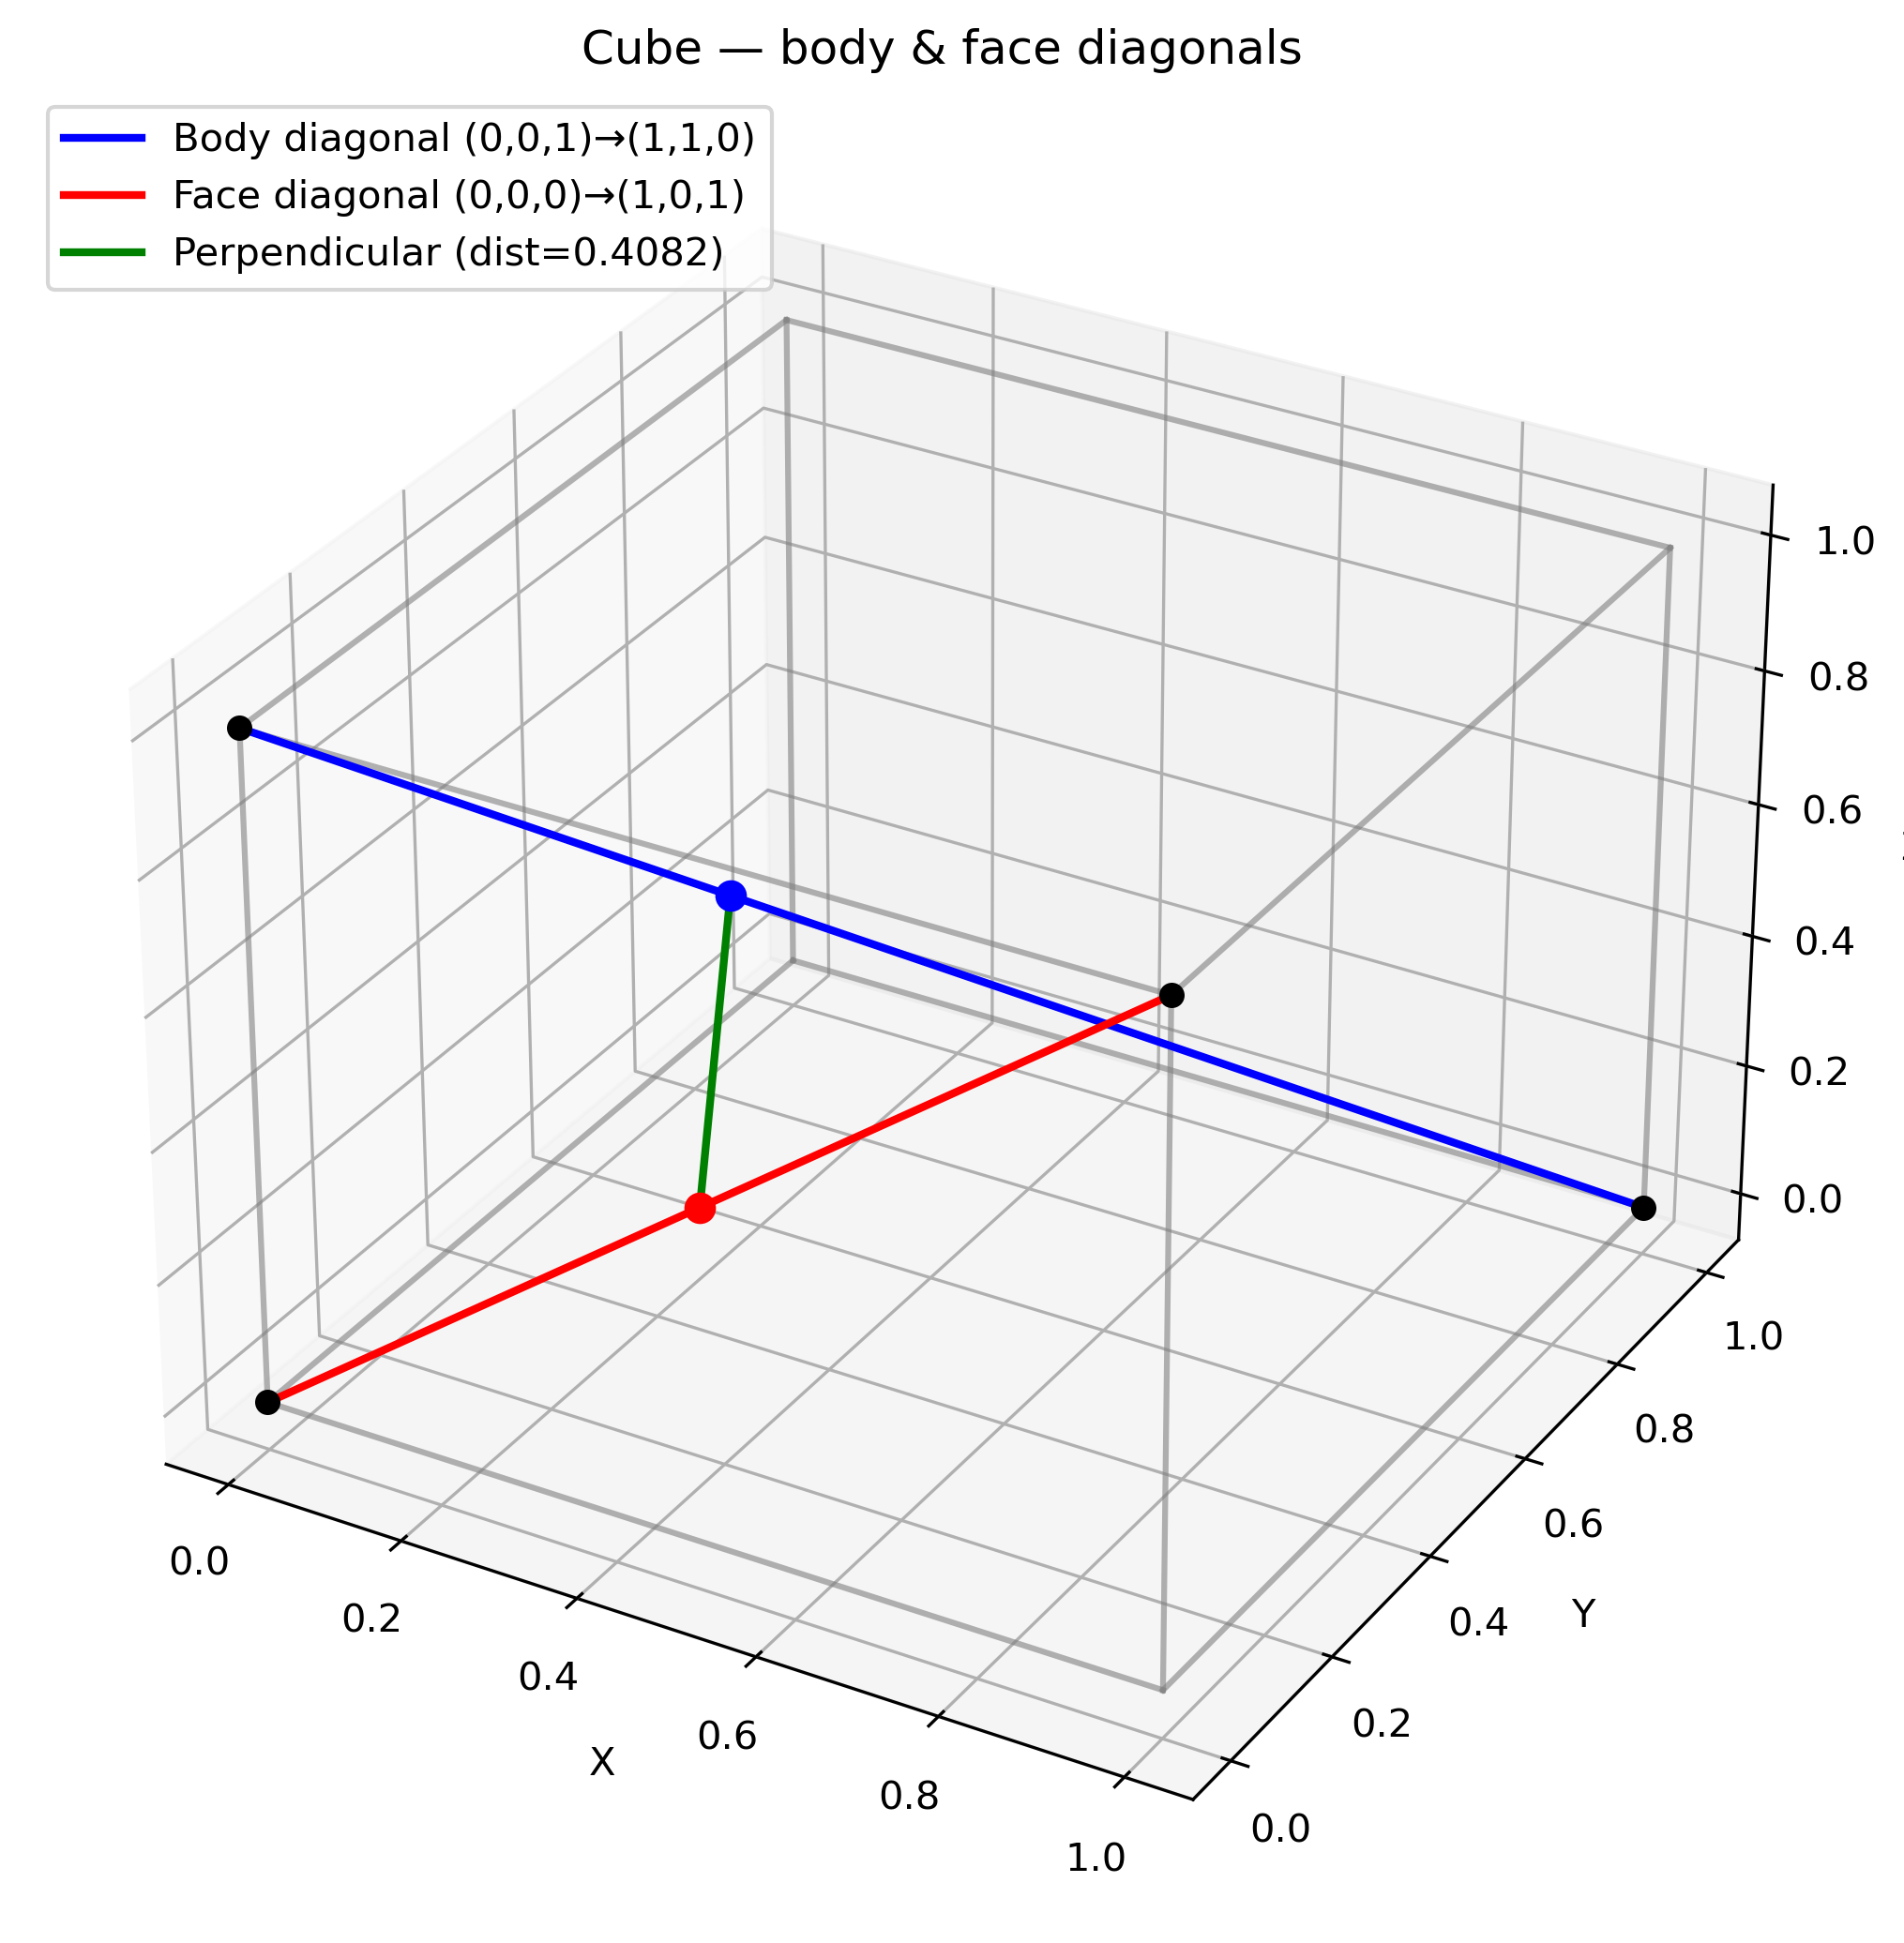
\includegraphics[width=0.7\columnwidth]{JEE/chapters/2.10.84/figs/cube_lines.png} 
   \caption{}
  \label{fig:2.10.84/Fig1}
\end{figure}

